%   File: robot_arm.tex
% Author: Adam Leeper
%------------------------------------------------------------------------------
%\\[0.45pc]
\providecommand{\isolatedBuild}[1]{#1}% fallback definition lets this file build normally
\isolatedBuild{
  \documentclass[11pt,letterpaper]{book}
  %\documentclass[11pt,letterpaper]{book}

% aleeper: I think these are needed for Paul's macros?
\usepackage{epsfig}
\usepackage{epstopdf}

%\makeatletter
%\typeout{The import path is \import@path}
%\makeatother

\usepackage{import}

\subimport{./}{packagesMitiguy.sty}
\subimport{./}{macrosMitiguy.tex}
\subimport{./}{PageStylesMitiguy.tex}
\subimport{./}{macrosLeeper.tex}
   % Must be found via TEXINPUTS environment variable.
  \isolatedBuildHeader{Vector Equations and Geometry}
                      {Position Kinematics of a Robot Arm}
}
%%%
%%%
%%%
Consider the robot arm shown. Frames A, B, C (shown) and frame N
(not shown) each have fixed in them right-handed, orthogonal unit
vectors \uvecBasisxyz{a}, \uvecBasisxyz{b}, \uvecBasisxyz{c}, and
\uvecBasisxyz{n}, respectively. The relevant lengths $L_1$, $L_2$,
and $L_3$ are shown on the drawing.
%
\\[0.45pc]
You are \textbf{given} the vector from a point $N_o$ (not shown) on the robot's base to the elbow point $A_o$ is
$\posvec{N_o}{A_o} = d_y~\uvecy{n} + d_z~\uvecz{n}$.
%
\begin{enumerate}
  \begin{minipage}[t]{0.5\linewidth}
    \item
      By inspection, write the position vector \textbf{from} the elbow
      point $A_o$ \textbf{to} the finger tip $Q$, using an efficient
      combination of basis vectors.
      %
      \\[0.5pc]
      $\posvec{A_o}{Q} \equals[\;]
      \hidemath[0cm]{L_1~\uvecx{a} + L_2~\uvecx{b} + L_3~\uvecy{c}}$
      \\[0.25pc]
      %
    \item
      Write the position vector from $N_o$ to $Q$, first as a sum of two or
      more \textbf{basis-independent} position vectors, then in terms of any
      given unit vectors.
      \\[0.5pc]
      $\posvec{N_o}{Q} \equals[\;]$
      $\posvec{\hidemath[0cm]{~\origin{A}~}}{\hidemath[0cm]{~~Q~}}
       \plus[\;]
       \posvec{\hidemath[0cm]{~\origin{N}~}}{\hidemath[0cm]{~\origin{A}~}}$
      %
      \\[0.45pc]
      $\posvec{N_o}{Q} \equals[\;]
      \hidemath[0cm]{d_y~\uvecy{n} \plus[\;] d_z~\uvecz{n} \plus[\;]
                     L_1~\uvecx{a} \plus[\;] L_2~\uvecx{b} \plus[\;]
                     L_3~\uvecy{c}}$
  \end{minipage}
  \hfill
  \begin{minipage}[t]{0.5\linewidth}
    \flushright
    \vspace*{-0.5pc}
    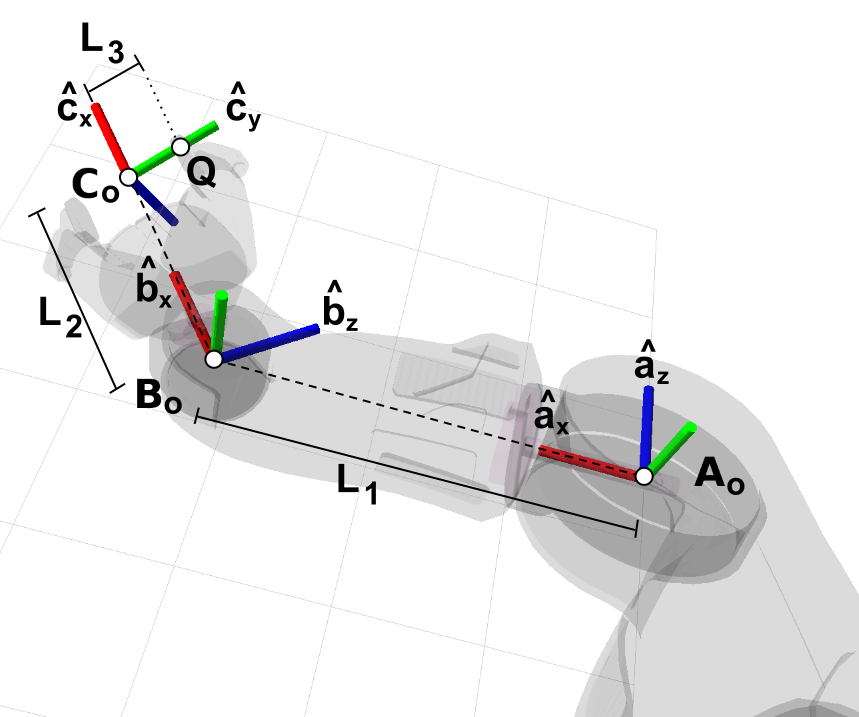
\includegraphics[width=0.9\linewidth]{arm_position.png}
  \end{minipage}
  %
  \item
    Your team-mate asks you for the ``x, y, z coordinates" of $Q$'s position
    from \origin{N} in frame \basis{N}. Explain/show which vector operations
    you would do to get these \textbf{measures} of \posvec{N_o}{Q}.
    (You do not need to complete the calculation; in fact, you don't have
    enough information to do so.)
    \\[0.45pc]
    \Solution {}{1.0\linewidth}{
      \uvecx{n} measure $ = (\uvecx{n} \DotProduct \posvec{N_o}{Q})$
      \\[0.2pc]
      \uvecy{n} measure $ = (\uvecy{n} \DotProduct \posvec{N_o}{Q})$
      \\[0.2pc]
      \uvecz{n} measure $ = (\uvecz{n} \DotProduct \posvec{N_o}{Q})$
      \\[0.45pc]
      \textbf{Note:} Can't complete the dot products, need rotation matrices
      relating the frames.
    }
  %
  \item
    A heavy ball held at $Q$ exerts a downward force
    $\force{Q} = -W~\uvecz{n}$ on the robot arm. Explain/show which (one)
    vector operation you would do to get the moment of this force about
    $A_o$, that is, $\moment{F^Q/A_o}$.
    \\[0.45pc]
    \Solution {}{1.0\linewidth}{
      $\moment{F^Q/A_o} \deff ~\posvec{Ao}{Q} \CrossProduct \force{Q}
       \equals[\;] (L_1~\uvecx{a} \plus[\;] L_2~\uvecx{b} \plus[\;]
       L_3~\uvecy{c}) \CrossProduct (-W~\uvecz{n})$
      \\[0.45pc]
      \textbf{Note:} Could distribute, but can't complete the cross products.
                  Need rotation matrices relating the frames.
    }
\end{enumerate}
%
\isolatedBuildFooter
